\documentclass[tikz,border=2pt]{standalone}
\begin{document}
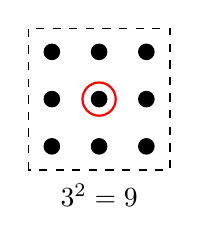
\begin{tikzpicture}[x=0.6cm,y=0.6cm]
  \foreach \i in {1,2,3} \foreach \j in {1,2,3} \fill (\i,\j) circle (3pt);
  \draw[dashed] (0.5,0.5) rectangle (3.5,3.5);
  \draw[red, thick] (2,2) circle (6pt);
  \node[below] at (2,0.4) {$3^2 = 9$};
\end{tikzpicture}
\end{document}
